%%%%%%%%%%%%%%%%%%%%%%%%%%%%%%%%%%%%%%%%%%%%%%%%%%%%%%%%%%%%%%%%%%%
% Method
% Team:
% Union
% Members: 
% Bernie Huang, Jim Lan, Hoang Tan, Kenny Hsu, Rahul Aditya, Tan Phat, Wei
% Relative files:
% Method_Union.tex
% Note:    
% Do not compile this file compile Main.tex to get the pdf file instead.
%%%%%%%%%%%%%%%%%%%%%%%%%%%%%%%%%%%%%%%%%%%%%%%%%%%%%%%%%%%%%%%%%%%
	
\subsection*{Title extraction}

\subsubsection*{Author abstraction}
\begin{itemize}
	\item I use the python to catch the abstract.
	\begin{center}
		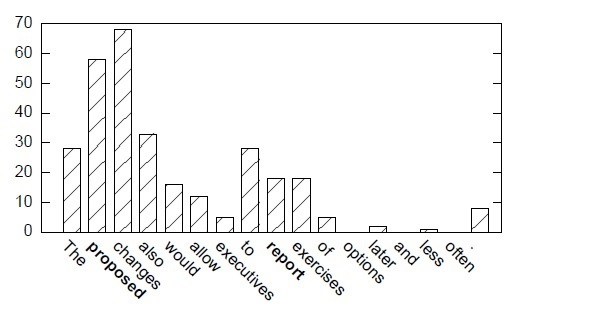
\includegraphics[width=0.8\columnwidth]{Union_Background_Chart_2}
	\end{center}
	\item Fist,the pdf be converted into txt.So it will create the txt file.\\ 
	\item Second,read the txt file every line.If the python detection the abstract-database's words ,it will start to catch the sentence.\\ 	
	abstract-database:include the condition\\
	    1. capital         "ABSTRACT"\\
	    2. lower case      "abstract"\\
	    3. in the sentence "Abstract—Word sense ....."\\
	    4. and so on \\
	\item Third,read the txt file every line.If the python detection the abstract-database-stop's words ,it will stop to catch the sentence.\\ 
    abstract-database-stop:include the condition
    1. the blank line
    2. specific word in the beginning "Keywords"
    3. and so on
	\item Fourth,output the sentence in the txt file\\ 	

\end{itemize}

\subsubsection*{Abstract extraction}

\nwepage
